\documentclass[12pt, titlepage]{article}

\usepackage{longtable}
\usepackage[utf8]{inputenc}
\usepackage{fullpage}
\usepackage{amsmath, mathtools}
\usepackage{amsfonts}
\usepackage{amssymb}
\usepackage{graphicx}
\usepackage{colortbl}
\usepackage{xr}
\usepackage{xr-hyper}
\usepackage{hyperref}
\usepackage{longtable}
\usepackage{xfrac}
\usepackage{tabularx}
\usepackage{float}
\usepackage{siunitx}
\usepackage{booktabs}
\usepackage{caption}
\usepackage{pdflscape}
\usepackage{fixltx2e}
\usepackage{afterpage}
\usepackage{seqsplit}
\usepackage{underscore}
\usepackage{lscape}
\usepackage[english]{babel}
\usepackage[T1]{fontenc}
\usepackage{booktabs}
\usepackage{tabularx}
\usepackage{hyperref}
\usepackage{nameref}
\usepackage{enumitem}


% checklist
\newlist{todolist}{itemize}{3}
\setlist[todolist]{label=$\square$}


\hypersetup{
    colorlinks,
    citecolor=blue,
    filecolor=black,
    linkcolor=red,
    urlcolor=blue
}
\usepackage[round]{natbib}
\MakeRobust{\ref}% avoid expanding it when in a textual label

\makeatletter
\newcommand{\labeltext}[2]{%
  \@bsphack
  \csname phantomsection\endcsname % in case hyperref is used
  \def\@currentlabel{#1}{\label{#2}}%
  \@esphack
}

% external references
%% Comments

\usepackage{color}

\newif\ifcomments\commentstrue %displays comments
%\newif\ifcomments\commentsfalse %so that comments do not display

\ifcomments
\newcommand{\authornote}[3]{\textcolor{#1}{[#3 ---#2]}}
\newcommand{\todo}[1]{\textcolor{red}{[TODO: #1]}}
\else
\newcommand{\authornote}[3]{}
\newcommand{\todo}[1]{}
\fi

\newcommand{\wss}[1]{\authornote{blue}{SS}{#1}} 
\newcommand{\plt}[1]{\authornote{magenta}{TPLT}{#1}} %For explanation of the template
\newcommand{\an}[1]{\authornote{cyan}{Author}{#1}}

%% Common Parts

\newcommand{\progname}{Mechatronics Engineering} % PUT YOUR PROGRAM NAME HERE
\newcommand{\authname}{Team \# 34, ParkingLotHawk
\\ Fady Zekry Hanna, zekryhf
\\ Winnie Trandinh, trandint
\\ Muhammad Ali, alim102
\\ Muhammad Khan, khanm120} % AUTHOR NAMES                  

\usepackage{hyperref}
    \hypersetup{colorlinks=true, linkcolor=blue, citecolor=blue, filecolor=blue,
                urlcolor=blue, unicode=false}
    \urlstyle{same}
                                

\externaldocument{../DevelopmentPlan/DevelopmentPlan}
\externaldocument{../HazardAnalysis/HazardAnalysis}
\externaldocument{../SRS/SRS}

\begin{document}

\title{Project Title: System Verification and Validation Plan for \progname{}} 
\author{\authname}
\date{\today}
	
\maketitle

\pagenumbering{roman}

\section{Revision History}

\begin{table}[hp]
\caption{Revision History} \label{TblRevisionHistory}
\begin{tabularx}{\textwidth}{llX}
\toprule
\toprule {\bf Date} & {\bf Version} & {\bf Notes}\\
\midrule
November 3, 2022 & 1.0 & Initial Revision \\
\bottomrule
\end{tabularx}
\end{table}

\newpage

\tableofcontents

\listoftables

\listoffigures

\newpage

\section{Symbols, Abbreviations and Acronyms}

\renewcommand{\arraystretch}{1.2}
\begin{tabular}{l l} 
  \toprule		
  \textbf{symbol} & \textbf{description}\\
  \midrule 
  T & Test\\
  \bottomrule
\end{tabular}\\

\wss{symbols, abbreviations or acronyms --- you can simply reference the SRS
  \citep{SRS} tables, if appropriate}

\wss{Remove this section if it isn't needed}

\newpage

\pagenumbering{arabic}

\section{General Information}

The Verification and Validation (VnV) Plan outlines the various methods that the team will conduct to verify and validate the ParkingLotHawk. The general overview of the plan can be found in \nameref{vnvPlan}, with detailed tests outlined within \nameref{systemTest} and \nameref{unitTest}.

\subsection{Summary}

The ParkingLotHawk is an autonomous aerial drone that helps parking lot operators understand the state of their parking lot. The drone shall be able of full autonomy, where it automatically explores the parking lot, or by semi-autonomy, where the operator specifies the locations that the drone should go to. During flight, the drone shall transmit live information about the parking lot sections it detects, and display this information to the operator. 

\subsection{Objectives}

There are multiple objectives to be accomplished for the proper operation of the drone. The following objectives will mainly focus on the most important qualities of the objectives:

\begin{itemize}
    \item Software Algorithm Correctness: The drone should be able to operate according to its specifications, and the application to be used by the operators should be able to accurately relay the commands to the drone.
    \item Hardware Correctness: The components of the drone functions properly according to their intended purpose and with minimal to no errors.
    \item State Machine Implementation: Control events exist and are correct for the various components of the drone in order to operate those specific parts individually.
    \item Operator's PC and Drone Communication: The components on the drone can accurately communicate with the operator application and the communication is functional during the entire time that the drone is functioning within the parking lot.
    \item Safety Features: The drone has a backup or failsafe code in the situation where any of its parts are malfunctioning or prior to the malfunction.
    \item Ease of Use: The operator should be able to properly understand how to operate the drone from the application, under the assumption that they only have basic knowledge of operating computers.
\end{itemize}

\subsection{Relevant Documentation}

In the remaining portion of the document, there will be various sources of information that will help verify the process for the product. The major sources will include the reference of the \href{https://github.com/icecap360/DroneCapstone/blob/master/docs/SRS/SRS.pdf}{SRS} and \href{https://github.com/icecap360/DroneCapstone/blob/master/docs/HazardAnalysis/HazardAnalysis.pdf}{HA} documents for the requirements, and the \href{https://github.com/icecap360/DroneCapstone/blob/master/docs/Design/MG/MG.pdf}{MG} and \href{https://github.com/icecap360/DroneCapstone/blob/master/docs/Design/MIS/MIS.pdf}{MIS} documents for the design.

\section{Plan}
\label{vnvPlan}

This section outlines the various methods that the team will use to verify and validate the components of the system. This includes verifying the SRS, design, VnV plan, and implementation. Automated testing and verification tools will also be presented to aid in the iterative verification process. Finally, methods for validating that the system solves the problem will be presented.

\subsection{Verification and Validation Team}

The members of the team are assigned an area of testing, where the area of testing is not their area of expertise. This ensures that the creator and tester are not the same person, which eliminates the bias that occurs when testing their own components. The assigned person to the testing area are then responsible for managing all tests in that domain. In the cases where a test covers multiple domains, the test will be conducted in a joint manner between the different domains. The assignment of the testing areas are indicated within \nameref{VnV_Team}.
  
\begin{table}[!h]
\begin{center}
\caption {Verification and Validation Team}
\label{VnV_Team}
\begin{tabular}{ | m{3cm} | m{3cm} | m{8cm} | }
\hline
Role & Name & Description \\
\hline
 Visual Perception and Path Planning & Fady & Verifies that the visual perception and autonomous exploration algorithm is performing within specifications. \\
\hline
Drone Finite State Machine (FSM) and Communication & Ali & Verifies that all communication between the drone components and the drone to the Operator's application are working correctly. \\
\hline
Mechanical Testing & Zaid & Verifies that all physical components and the dynamics are working within specifications. \\
\hline
Operator's Application & Winnie & Verifies that the Operator's application and user manual meet the specifications outlined.
\\
\hline
\end{tabular}
\end{center}
\end{table}

\clearpage

\subsection{SRS Verification Plan}
\label{SRSVerification}

To verify the SRS, both formal and informal processes will be conducted. To test the completeness of the FSM, a formal decision table shall be created and maintained. This process ensures that all transitions and external stimuli are accounted for, in addition to identifying any states that cannot be reached or cannot be exited. The initial decision table has already been created within the SRS, located in \nameref{appendixb}. To verify that the decision table is accurate as the project progresses, this table will be updated with any changes to the FSM. 

To informally verify the other components of the SRS, guided reviews and a checklist shall be conducted. The guided review will consist of the team explaining the Functional Requirements to a technical external party, and the external party will list any potential NFRs that are related to the FR. The team shall then ensure that the NFR is present within the SRS. Furthermore, the team shall have other capstone groups review the SRS using the provided rubric as guidelines for the review. The last method is to conduct a checklist, conducted either internally within the team or by an external party. The checklist is as follows: 

\begin{todolist}
\label{SRS_Checklist}
\item For each requirement within the SRS, are the following met?
\begin{todolist}
    \item Does the requirement address a specific goal?
    \item Is the requirement unique? 
    \item Is the requirement abstract?
    \item Is the requirement traceable?
    \item Is the requirement complete?
    \item Is the requirement measurable?
    \item Are there no inputs that are not used in the determination of the output? 
    \item Does each output use at least one input, and are all required inputs listed?
\end{todolist}
\item Does the Finite State Machine comply with the following?
\begin{todolist}
    \item Are all states unique?
    \item Are all states complete, and should not be combined or split into multiple states?
    \item Are all error states included?
    \begin{todolist}
        \item Are all data exceptions accounted for?
        \item Are error logging and recovery mechanisms present?
    \end{todolist}
    \item Are all transitions mutually exclusive?
    \item Are all state names meaningful and representative of the state?
\end{todolist}
\end{todolist}

\subsection{Design Verification Plan}

The team plans to verify the design through structured review processes and a checklist. The review shall consist of the team explaining the product and design to an external party, and providing the external party with the FRs. They will then ensure that all the FRs are met, by using the checklist as a reference. The checklist is as follows, with additional detail on the requirements available in \nameref{sec:funcReqs}: 

\begin{todolist}
\label{Design1_Checklist}
\item Does the design implement all the general function requirements listed below?
\begin{todolist}
    \item The product shall be able to recognize Clear Boundaries.
    \item The product shall provide live update of c\_CurrentLoc, c\_CurrentView and c\_OccupancyMap during all normal and non-configurational operation states.
    \item The product shall allow the operator to configure the i\_MinHoverHeight, i\_MaxHoverHeight, and i\_DesiredHoverHeight.
    \item The condition i\_MinHoverHeight <= i\_DesiredHoverHeight <= i\_MaxHoverHeight shall always be true.
    \item The product shall be able to identify non-occupied parking spots.
    \item The product shall be shall highlight non-occupied parking slots on the operator's display (update c_CurrentView).
\end{todolist}
\item Does the design implement all the state implementation requirements listed below?
\begin{todolist}
    \item The product shall implement an Idle state.
    \item The product shall implement a Hover State.
    \item The product shall implement a Manual Move State.
    \item The product shall implement an Autonomous Explore State.
    \item The product shall implement a Configure state.
    \item The product shall implement an Off state.
    \item The product shall implement a Land state.
    \item The product shall implement a Desired Location Error state.
    \item The product shall implement a No Parking Lot Detected Error state.
    \item The product shall implement a Malfunction state.
    \item The product shall implement a Communication Lost state.
    \item The product shall implement a Compulsive Move State.
\end{todolist}
\item Does the design implement all the state transition requirements listed below?
\begin{todolist}
    \item Upon the m\_PowerOn becoming false, the drone shall enter the Off state.
    \item Upon the m\_PowerOn becoming true, the drone shall enter the Idle state.
    \item Upon the m\_Launch becoming true, the drone shall enter the Hover state if the i\_Mode was set to normal, and enters the Configure state if the i\_Mode was set to configure.
    \item If in the Hover state, and c\_ParkingLotDetected is equal to true, the product shall enter the Autonomous Explore state and explore the detected lot.
    \item Once the user enters or changes m\_DesiredUserLoc and m\_CompulsiveMove is asserted as false, the drone shall automatically enter the Manual Move state.
    \item If while in the Manual Move state and the product determines that m\_DesiredUserLoc is outside parking lot boundaries, the product shall enter the Desired Location Error state.
    \item When m\_AutonomousExplore is set to true and c\_ParkingLotDetected is equal to true, the product shall enter the Autonomous Explore state.
    \item When m\_AutonomousExplore is set to true but c\_ParkingLotDetected is equal to false, the product shall enter the No Parking Lot Detected Error state.
    \item Upon m\_Land being true, the product shall enter the Land state.
    \item If c\_Connected becomes false for more than 5 seconds, or signal strength (dBm) has lost 80\% of its typical value at any point during operation, then the product shall enter the Communication Lost state.
    \item If while in the Communication Lost State, c\_Connected becomes true for more than 5 seconds, or signal strength (dBm) has returned to 50\% of its typical value at any point during operation, then the product shall enter the Hover state.
    \item Once the user enters or changes m\_DesiredUserLoc and m\_CompulsiveMove is asserted as true, the drone shall automatically enter the Compulsive Move state.
\end{todolist}
\end{todolist}

Internally within the team, a more detailed checklist shall be conducted that includes all the requirements listed within the SRS. To exclude any biases from the creator of the modules, the creator and tester will not be the same when conducting this review. Therefore, the members listed within section [xx] will be responsible for reviewing the requirements within their section. This ensures that all the requirements are accounted for within the design. The full checklist consists of the checklist above, in addition to the following: 

\begin{todolist}
\label{Design2_Checklist}
\item Does the design implement all the performance requirements listed below?
\begin{todolist}
    \item The product shall explore up to 1400 $m^2$ of the detected parking lot during the Autonomous Explore State.
    \item The product shall takeoff to i\_MaxHoverHeight and land from i\_MaxHoverHeight within 25 seconds.
    \item The product shall move to a specified location with an average speed exceeding 4km/hour.
    \item The product shall transmit all data to the operator at a rate exceeding 0.5 frames per second.
    \item The product shall maintain a longitudinal and lateral position within a 1.5m radius during the Hover State.
    \item While the product is not hovering (moving from one location to another), it shall always maintain an altitude between i\_MaxHoverHeight and i\_MinHoverHeight, within a tolerance of ±5\%.
    \item The product shall be operable within requirements within non-inclement weather.
    \item The product shall maintain a longitudinal and lateral position within a 1.5m radius once the product has reached m\_DesiredUserLoc while in the Manual Move State or Compulsive Move State.
\end{todolist}
\item Does the design implement all the design constraints listed below?
\begin{todolist}
    \item The product shall cost less than \$750 to manufacture.
\end{todolist}
\item Does the design implement all the standards and compliance requirements listed below?
\begin{todolist}
    \item The product shall weigh a total of less than 25kg.
    \item The product shall use radio communication only within the 2.4 GHz or 900 MHz range.
\end{todolist}
\item Does the design implement all the security requirements listed below?
\begin{todolist}
    \item The operator's application shall only be launched by a user with authorized access.
    \item The product shall not upload any gathered data to any external parties.
\end{todolist}
\item Does the design implement all the maintainability requirements listed below?
\begin{todolist}
    \item The product shall be fully recharged within 1 hour.
    \item The product shall be able to sustain a fall of greater than 1m without sustaining damage that affects operation performance.
    \item The product shall be mechanically waterproof, to the point it can sustain a light drizzle for 1 minute of operation while still performing within the requirements.
\end{todolist}
\item Does the design implement all the safety requirements listed below?
\begin{todolist}
    \item The product shall not influence or interact with dynamic actors positioned in the parking lot.
    \item The product shall not allow the operator to set i\_MaxHoverHeight, i\_MinHoverHeight, or i\_DesiredHoverHeight to be below 7m.
    \item The product shall not require the operator to physically manipulate the product in any way in any state outside of Off State.
    \item The product shall not cause distractions or negatively impact greater than 2\% of the visitors in the parking lot.
    \item The product shall include a mechanical Off switch to the product.
\end{todolist}
\item Does the design implement all the usability requirements listed below?
\begin{todolist}
    \item The product shall provide a visual trace of its location for the past 60 seconds +- 1 second.
    \item The product shall allow the operator to save the current visual and raw data into a folder.
    \item The product shall be able to operate and provide data to the operator for > 5 minutes without the need to recharge.
    \item The product shall require less than 2 hours of training for the operator to use.
    \item The product shall display the current state to the Operator's PC Application.
\end{todolist}
\end{todolist}

\subsection{Verification and Validation Plan Verification Plan}

The Verification and Validation Plan shall be verified through an informal peer review process and a checklist. The peer review shall be conducted by another technical Capstone group and will use the provided rubric as a guideline. The checklist can then be conducted either internally within the team, or by an external party. The checklist is as follows, and ensures that all components of the VnV Plan are present: 

\begin{todolist}
\label{VnV_Checklist}
\item Are methods outlined to verify the SRS and the requirements within it?
\begin{todolist}
    \item Are all requirements covered by system tests?
\end{todolist}
\item Are methods outlined to verify the design?
\item Are methods outlined to verify the implementation of the design?
\item Are automated testing and verification tools clearly outlined and feasible?
\item Are methods outlined to validate the design and ensure that it solves the problem statement?
\item Are all methods outlined in the VnV Plan feasible, given the current resources available for VnV?
\item Is there traceability between the test plans and the requirements?
\item Are tests outlined specifically and clearly, such that they can be reproduced by an external party?
\end{todolist}


\subsection{Implementation Verification Plan}

The implementation shall be verified primarily by the tests outlined within sections [xx] and [xx]. These sections include a combination of static, dynamic, and stress tests to ensure that the system is meeting the requirements of the system. Furthermore, the team shall conduct a code walkthrough for the FSM implementation. Conducted within the team, the implementor of the FSM shall provide the code used, and explain the state and transitions implemented. Using just the code, the team shall then recreate the entire FSM model as shown within the SRS at [here]. This process ensures that the implementation of the FSM matches the required FSM exactly.  

The team shall also conduct code reviews of the changes before the changes are merged into the master branch within GitHub. This ensures that a peer review process is implemented as part of the GitHub management system and that the changes are correct. In addition to the code walkthroughs, automated testing and verification tools shall also be used to verify the implementation of the system, as outlined within \nameref{automatedVerificationTools}. 


\subsection{Automated Testing and Verification Tools}
\label{automatedVerificationTools}

The team shall implement a variety of tools to automate the testing and verification process. Discussed upon within the \nameref{codingStandard}, the team shall use a common IDE within the team, with integrated linters for both Python and C++. This ensures that static analyzers and coding standards are implemented automatically by the IDE and linter. A unit testing framework shall also be used to aid in the testing of the modules. Due to the usage of ROS within the product, the team shall use GTest for C++ modules, UnitTest for Python modules, and RosTest for ROS specific modules and communication. These three frameworks directly integrate within the ROS workflow, allowing for automatic execution of these tests during the compilation of the ROS packages. To further aid in the compilation of the various ROS packages, CMake shall be used to automate and simplify the compilation process. In addition to these tools, the team shall also produce a custom testing framework to test the visual perception algorithms. The custom tool shall automate the process of feeding in hardcoded input images into the algorithm, and record the algorithm outputs within a CSV file for easy manipulation and analysis of the outputs. 

\subsection{Software Validation Plan}

The system shall be verified by two main methods. A guided review process shall be conducted by an external party, where the team provides and explains the FRs to the external party. They will then determine what the problem statement is, without the actual problem statement being provided by the team. This ensures that the SRS solves the given problem. To verify that the SRS has been met, the \nameref{SRSVerification} will be used. To further test the functionality of the visual perception, open source datasets shall be used, in addition to the testing methods outlined within \nameref{automatedVerificationTools}. Two open source datasets will be used: the \href{https://www.kaggle.com/datasets/blanderbuss/parking-lot-dataset}{Blanderbuss dataset} and the \href{http://cnrpark.it/}{CNRPark dataset}. Sample images of these datasets are shown within Figures \ref{BlanderbussSample} and \ref{CNRParkSample}. These datasets will then verify the performance of the system with regards to the parking lot detection and occupancy in a variety of different conditions.  

\begin{figure}[h!]
  \begin{center} 
  \caption{Blanderbuss Dataset Sample}
  \label{BlanderbussSample}
        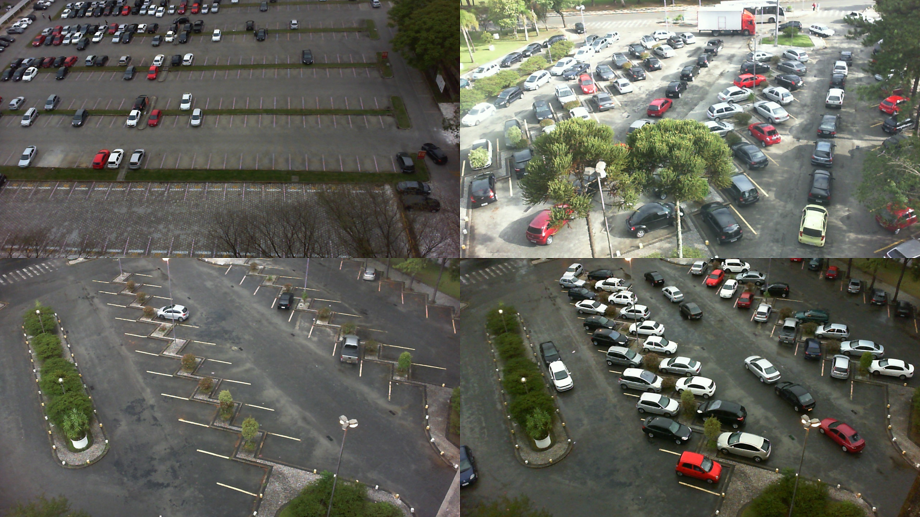
\includegraphics[width=1\textwidth]{VnVPlan/BlanderbussDataset.png}
  \end{center}
\end{figure}

\begin{figure}[h!]
  \begin{center} 
  \caption{CNRPark Dataset Sample}
  \label{CNRParkSample}
        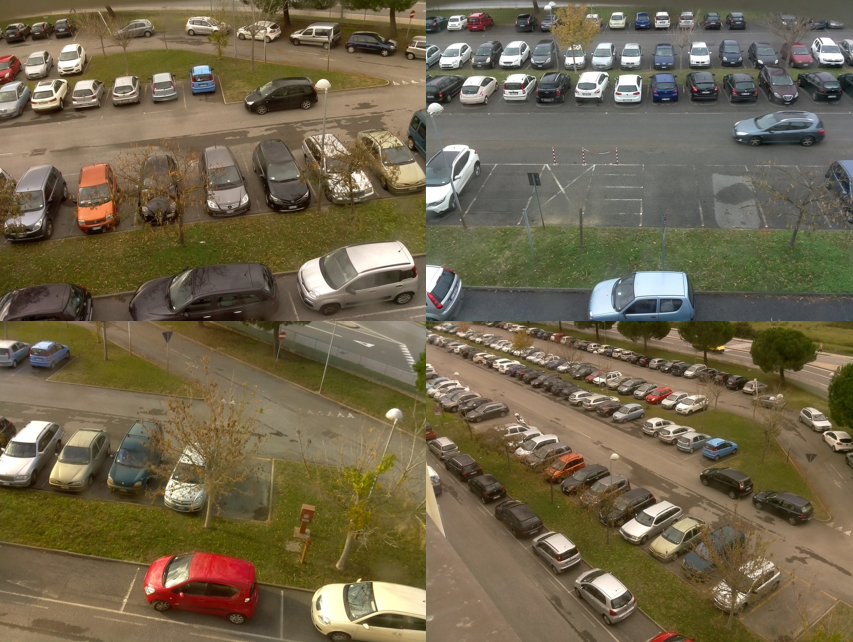
\includegraphics[width=1\textwidth]{VnVPlan/CNRParkDataset.png}
  \end{center}
\end{figure}

\clearpage

\section{System Test Description}
\label{systemTest}

\subsection{Measuring Outputs Testing}

There are several ways to measure the output variables. Some suggestions are given in the following section. 

In general, given that all output variables can be viewed using the Operator's Application, this is perhaps the easiest source to measure the drone's response. There are special systems and unit tests to verify if the Operator's Application is correctly displaying/gathering the output variable.

Another method of viewing output variables is to print and store the output variables in log files within the onboard drone computer's file system. They can then be collected or sent to the Operator's PC to analyze the logs later.

To collect time statistics, either the timer on the embedded computer can be used and printed in log files, or one can use an external manual timer.

For all test cases, to measure location and height, the GPS location and height displayed on the Operator's PC Application can be used, except for the Flight Dynamics Tests \ref{flightdynamicsTests}, in these scenarios an external location and height measurement tool must be used. Examples to measure lateral location include adding an external and light GPS to the drone or walking underneath the drone with an external GPS (like the ones on smart phones). To measure height one may use marks on a wall, or even attach a rope to the drone.

\subsection{Assumptions regarding test cases}
Unless otherwise stated, the test case requires that there is enough battery to complete the test case.
Unless the creation of special stubs is specified, the drone is assumed to be complete mechanically, electrically, and software-wise. 

\subsection{Tests for Functional Requirements}

The test cases were designed to for coverage over all the requirements that needed testing for verification. Requirements are grouped into the system component that is most difficult or most central to the task. However there is overlap between the test case categories, for example, the User Error Test Cases \ref{usererrorTests} utilize the Visual Perception component to make decisions/transitions.

\subsubsection{Flight Dynamics}
\label{flightdynamicsTests}

\begin{table}[!h]
\begin{center}
\caption {STC\_001}
\label{tab:STC_001}
\begin{tabular}{ | m{1.5cm} | m{15cm} | } 
\hline
ID & \nameref{tab:STC_001} \\ 
\hline
Control & Manual \\ 
\hline
Initial State & The product is in its Off state. \\ 
\hline
Input & Enter the configure state and set \ref{Indoor_Hover_Params}. Afterwards, launch the drone in normal operation and wait for 1 min 25 sec. \\ 
\hline
Output & The drone should take less than 25 seconds to reach and hover within 1 +- 0.5 m from the moment the drone launches. While hovering, the drone should laterally stay within a 1.5 m radius of the launch location. \\ 
\hline
How test will be performed & A stub must be created in the code to suppress the requirement of the hover parameters being at least \ref{Min_Hover_Params}, as indoor conditions permit only a much lower flight height. 

The first step of the test, configuring height parameters, is accomplished by:
\begin{enumerate}[topsep=0pt,itemsep=-1ex,partopsep=1ex,parsep=1ex]
    \item Setting the input i\_Mode as Configure and turning the power switch of the drone to On.
    \item Assert m\_Launch, so the drone enters the Configure state.
    \item Setting the height parameters in the Operator's PC Application to \ref{Indoor_Hover_Params}.
\end{enumerate}
The second step of the drone, having the drone enter and stay within the hover state, is accomplished by:
\begin{enumerate}[topsep=0pt,itemsep=-1ex,partopsep=1ex,parsep=1ex]
	\item Turning the power switch on the drone off. Then set i\_Mode as Normal and turn the power switch on, so the drone enters Idle state.
	\item Placing the drone in a non-parking lot area. 
	\item Asserting m\_Launch as true, then wait for 25 sec.
	\item Wait for 1 min. During this wait measure the output variables.
\end{enumerate}
Once the output variables have been measured and the test is complete, assert m_Land to true so the drone transitions to the land state.\\ 
\hline
Test case derivation & As per SRS, while in the Hover state, the drone will enter the Autonomous Explore state if it sees a parking lot. The purpose of placing the drone in a non-parking lot area was to keep the drone in the Hover state rather than entering the Autonomous Explore state.

While hovering the drone should stay within a 1.5 m radius laterally, without the presence of any external forces such as wind.

This test is an extension of STC_001, where this test is conducted within a controlled environment, and STC_001 is conducted within the actual environment with external forces. \\ 
\hline
Purpose of test and/or relationship to other tests &  • Assesses and verifies the flight dynamics in an indoor scenario, which won't have the gusts and winds of outdoor test cases.

• Verifies the states Off, Idle, Hover, Configure and Land as well as the transitions between them. In particular, it verifies NFR requiring the drone to stay within a 1.5m radius within the hover state (\nameref{STA_000}, \nameref{STA_001}, \nameref{STA_004}, \nameref{STA_005}, \nameref{STA_006}, \nameref{TRANS_002}, \nameref{TRANS_003}, \nameref{TRANS_009}).

• Verifies a corner case in the parking lot detection algorithm, that it correctly detects no parking lot when there is no parking lot (\nameref{GEN_001}).

• Elucidates how the drone operates in a non-parking lot area.
\\ 
\hline
\end{tabular}
\end{center}
\end{table}

\begin{table}[!h]
\begin{center}
\caption {STC\_002}
\label{tab:STC_002}
\begin{tabular}{ | m{1.5cm} | m{15cm} | } 
\hline
ID & \nameref{tab:STC_002} \\ 
\hline
Control & Manual \\ 
\hline
Initial State & The product is in its Off state. \\ 
\hline
Input & Enter the configure state and set the hover height parameters to be the smallest values possible value \ref{Min_Hover_Params}. Afterward, launch the drone in normal operation and wait for 1 min 25 sec. \\ 
\hline
Output & From the moment of launch, it should take less than 25 seconds to reach and hover within 7+-1.5 m. While hovering, the drone should laterally stay within a 1.5 m radius of the launch location, and it should stay within 5.5m and 8.5m above the ground at all times. \\ 
\hline
How the test will be performed & 
The first step of the test, configuring height parameters, is accomplished by:
\begin{enumerate}[topsep=0pt,itemsep=-1ex,partopsep=1ex,parsep=1ex]
    \item Setting the input i\_Mode as Configure and turning the power switch of the drone to On.
    \item Assert m\_Launch, so the drone enters the Configure state.
    \item Setting the height parameters in the Operator's PC Application to \ref{Min_Hover_Params}.
\end{enumerate}
The second step of the drone, having the drone enter and stay within the hover state, is accomplished by:
\begin{enumerate}[topsep=0pt,itemsep=-1ex,partopsep=1ex,parsep=1ex]
	\item Turning the power switch on the drone off. Then Setting i\_Mode as Normal and turning the power switch on so the drone enters the Idle state.
	\item Placing the drone in a non-parking lot area. 
	\item Asserting m\_Launch as true, then wait for 25 sec.
	\item Wait for 1 min. During this wait, measure the output variables.
\end{enumerate}
Once the output variables have been measured and the test is complete:
Assert m\_Land to true so that drone will enter the land state.\\ 
\hline
Test case derivation & As per SRS, the smallest possible height parameters are \ref{Min_Hover_Params}. 

As per SRS, the drone should take less than 25 seconds to reach i\_MaxHoverHeight (7+-1.5 m) from the moment the drone launches. This is why the input steps specify a 25-second wait after launch.

As per SRS, while in the Hover state, the drone will enter the Autonomous Explore state if it sees a parking lot. Thus, a non-parking lot area is used to prevent this transition.

While hovering, the drone should stay within a 1.5m lateral radius, with a height within i\_MaxHoverHeight-1.5m=7-1.5=5.5m and i\_MaxHoverHeight+1.5m=7+1.5=8.5m above the ground.  
\\ 
\hline
Purpose of test and/or relationship to other tests & This verifies that the configure state can change flight parameters in accordance with the restrictions specified in the SRS (\nameref{GEN_003}, \nameref{GEN_004}).
Elucidates how the drone operates in a non-parking lot area.
Verifies that the drone's flight dynamics are accurate, to the point that it can fly at the minimum height while maintaining minimum height safety requirements.
Verifies the states Off, Idle, Hover, Configure, and Land as well as the transitions between them. In particular, it verifies the NFR requiring the drone to stay within a 1.5m radius within the hover state (\nameref{STA_000}, \nameref{STA_001}, \nameref{STA_004}, \nameref{STA_005}, \nameref{STA_006}, \nameref{TRANS_002}, \nameref{TRANS_003}, \nameref{TRANS_009}).
Verifies a corner case in the parking lot detection algorithm, where it correctly detects no parking lot when there is no parking lot.
Verifies the NFR requiring the product to take off to i\_MaxHoverHeight within 25 seconds (\nameref{PERF_002}). \\ 
\hline
\end{tabular}
\end{center}
\end{table}

\begin{table}[!h]
\begin{center}
\caption {STC\_003}
\label{tab:STC_003}
\begin{tabular}{ | m{1.5cm} | m{15cm} | } 
\hline
ID & \nameref{tab:STC_003}  \\ 
\hline
Control & Manual\\ 
\hline
Initial State & The product is in its Off state.
 \\ 
\hline
Input & Enter the configure state and set the hover height parameters to be \ref{Med_Hover_Params}. Afterward, launch the drone in normal operation and wait for 1 min 25 sec. \\ 
\hline
Output & The drone should take less than 25 seconds to reach and hover within 7+-1.5 m from the moment the drone launches. While hovering, the drone should laterally stay within a 1.5 m radius of the launch location, and it should stay within 18.5m and 21.5m above the ground at all times. 
 \\ 
\hline
How test will be performed &
The first step of the test, configuring height parameters, is accomplished by:
\begin{enumerate}[topsep=0pt,itemsep=-1ex,partopsep=1ex,parsep=1ex]
    \item Setting the input i\_Mode as Configure and turning the power switch of the drone to On.
    \item Assert m\_Launch, so the drone enters the Configure state.
    \item Setting the height parameters in the Operator's PC Application to \ref{Med_Hover_Params}.
\end{enumerate}
The second step of the drone, having the drone enter and stay within the hover state, is accomplished by:
\begin{enumerate}[topsep=0pt,itemsep=-1ex,partopsep=1ex,parsep=1ex]
	\item Turning the power switch on the drone off. Then set i\_Mode as Normal and turn the power switch on, so the drone enters Idle state.
	\item Placing the drone in a non-parking lot area. 
	\item Asserting m\_Launch as true, then wait for 25 sec.
	\item Wait for 1 min. During this wait measure the output variables.
\end{enumerate}
Once the output variables have been measured and the test is complete:
Assert m\_Land to true, so that drone will enter the land state.\\ 
\hline
Test case derivation & As per SRS, the drone should take less than 25 seconds to reach i\_MaxHoverHeight (20+-1.5 m) from the moment the drone launches. This is why the input steps specify a 25 sec wait after launch.

As per SRS, while in the Hover state, the drone will enter the Autonomous Explore state if it sees a parking lot. The purpose of placing the drone in a non-parking lot area is to keep the drone in the Hover state.

While hovering the drone should stay a 1.5 m radius. In terms of height, it means that the drone should hover within i\_MaxHoverHeight-1.5m=20-1.5=18.5m and i\_MaxHoverHeight+1.5m=20+1.5=21.5m above the ground.  \\ 
\hline
Purpose of test and/or relationship to other tests & This test is very similar to \nameref{tab:STC_001}, except that the height parameters are configured to be much higher. The purpose of configuring the height parameters differently is to verify that the drone can hover accurately at different heights, that the drone can land safely from different heights, and that the Configure state is actually capable of configuring the height variables (\nameref{GEN_003}, \nameref{GEN_004}).

Verifies the states Off, Idle, Hover, Configure, and Land as well as the transitions between them. In particular, it verifies the NFR requiring the drone to stay within a 1.5m radius within the hover state (\nameref{STA_000}, \nameref{STA_001}, \nameref{STA_004}, \nameref{STA_005}, \nameref{STA_006}, \nameref{TRANS_002}, \nameref{TRANS_003}, \nameref{TRANS_009}). 
Verifies a corner case in the parking lot detection algorithm where it correctly detects no parking lot when there is no parking lot.
Elucidates how the drone operates in a non-parking lot area.
Verifies the NFR requiring the product to take off to i\_MaxHoverHeight within 25 seconds (\nameref{PERF_002}). \\ 
\hline
\end{tabular}
\end{center}
\end{table}

\begin{table}[!h]
\begin{center}
\caption {STC\_004}
\label{tab:STC_004}
\begin{tabular}{ | m{3.2cm} | m{12.2cm} | } 
\hline
ID & \nameref{tab:STC_004} \\ 
\hline
Control & Manual \\ 
\hline
Initial State & The product is in any of its flying states.   \\ 
\hline
Input & Set m\_CompulsiveMove as false. Change m\_DesiredUserLoc to a location within the parking lot and to the diagonal front right of the drone at least 20m away.  \\ 
\hline
Output & The drone should enter the Manual Move state upon a change to m\_DesiredUserLoc. The drone should move to and stay within 1.5m radially of the specified location. 
The user should also see a visual trace of the drone's movement; it should be a roughly straight line (shortest path).
Measure the time takes to reach the specified GPS location and calculate the average speed. As per SRS, ensure it is more than 4 m/sec.  \\ 
\hline
How test will be performed & Input section contains enough detail. \\ 
\hline
Test case derivation & As per SRS, the drone should enter Manual Move state whenever m\_DesiredUserLoc is changed and m\_CompulsiveMove is false. In this state the drone should travel to m\_DesiredUserLoc and hover with an accuracy of 1.5m. 

A visual trace of the drone's movement in the past 60 seconds should be displayed on the Operator's PC Application. It should appear as a relatively straight diagonal line toward the hover location, as the drone's path planning should make it take the shortest path. 

Using the time taken, the average speed of the drone can be calculated as distance/time. As per the SRS, it should be at least 4 m/sec. 
 \\ 
\hline
Purpose of test and/or relationship to other tests & 
\begin{itemize}
    \item Assesses the ability of the drone to move to forward as well as move rightward in a stable and efficient manner toward a specified GPS location.
    \item Helps verify the Manual Move state and transitions related to proceeding to a given location when the location is within the parking lot (\nameref{STA_002}, \nameref{TRANS_005}).
    \item Verifies the NFRs related to lateral accuracy (\nameref{PERF_008}. 
    \item Verifies the visual trace requirement (\nameref{USE_001}. 
    \item Verifies the average speed requirement (\nameref{PERF_003}. 
\end{itemize}
\\ 
\hline
\end{tabular}
\end{center}
\end{table}

\clearpage

\subsubsection{Battery}


\begin{table}[!h]
\begin{center}
\caption {STC\_005}
\label{tab:STC_005}
\begin{tabular}{ | m{3.2cm} | m{12.2cm} | } 
\hline
ID & \nameref{tab:STC_005} \\ 
\hline
Control & Manual \\ 
\hline
Initial State & The product is in the Idle state. \\ 
\hline
Input & Record the remaining battery stated on the Operator's PC Application. Disconnect the battery from the drone and connect it to the battery charger and record the remaining battery levels it detects. \\ 
\hline
Output & Battery levels stated on the Operator's Application should match the battery levels stated on the battery charger. \\ 
\hline
How test will be performed & Input section contains enough detail. \\ 
\hline
Test case derivation & As per HA, the drone should display the remaining battery on the Operator's PC Application. \\ 
\hline
Purpose of test and/or relationship to other tests & Verification that the display of the remaining battery on the Operator's PC Application is accurate (\nameref{SR_003}). \\ 
\hline
\end{tabular}
\end{center}
\end{table}

\begin{table}[!h]
\begin{center}
\caption {STC\_006}
\label{tab:STC_006}
\begin{tabular}{ | m{3.2cm} | m{12.2cm} | } 
\hline
ID & \nameref{tab:STC_006} \\ 
\hline
Control & Manual \\ 
\hline
Initial State & The product is in its Idle state. The drone battery is fully charged. \\ 
\hline
Input & To launch the drone, assert m\_Launch as true. Let the drone operate in any flying state. \\ 
\hline
Output & Observe the battery levels displayed on the Operator’s Application fall with time. It should fly in normal operation for at least 3.5 minutes.
At some point, the battery will be running very low (less than 1.5 minutes of flight left) and the drone will automatically enter the Malfunction state. In this state an error message will be logged to c\_Log, the c\_HealthStatus is set to Unhealthy, and the drone returns to the launch location. \\ 
\hline
How test will be performed & Regarding the initial state, verifying that the battery capacity is full can be accomplished by using the battery's charger. Input steps are self-explanatory. \\ 
\hline
Test case derivation & As per SRS, the Malfunction state must send an error message to c\_Log, change the c\_HealthStatus to Unhealthy, and the drone returns to the launch location.
As per HA, the drone must enter the Malfunction state and land itself when the remaining battery is detected to be low (less then 1.5 minutes). As per SRS, the drone must have a total battery capacity of lasting at least 5 minutes, leading to at least 3.5 minutes of flight.
As per HA, the drone must display the amount of battery remaining to the operator. 
 \\ 
\hline
Purpose of test and/or relationship to other tests & 
\begin{itemize}
    \item Verification of the low battery transition to the malfunction state (\nameref{SR_011}). 
    \item Verification of the operation of the malfunction state and transition into it (\nameref{STA_009}).
    \item Verification of the NFR requiring flight time to be at least 5 minutes (\nameref{USE_003}). 
    \item Verification of the FR requiring the drone to display remaining battery life to the operator (\nameref{SR_003}). 
\end{itemize}
\\ 
\hline
\end{tabular}
\end{center}
\end{table}

\begin{table}[!h]
\begin{center}
\caption {STC\_007}
\label{tab:STC_007}
\begin{tabular}{ | m{3.2cm} | m{12.2cm} | } 
\hline
ID & \nameref{tab:STC_007} \\ 
\hline
Control & Manual \\ 
\hline
Initial State & The product is in its Idle state. The drone has less than 3 minutes of battery remaining.  \\ 
\hline
Input & Attempt to launch the drone via setting m\_Launch as true. \\ 
\hline
Output & Drone should not launch, and instead, a descriptive error should be logged into the variable c\_Log.  \\ 
\hline
How test will be performed & Input section contains enough detail. \\ 
\hline
Test case derivation & As per HA, the drone should not fly unless there is more the 3 minutes of battery remaining.
 \\ 
\hline
Purpose of test and/or relationship to other tests & Verification of the FR requiring the drone to not fly unless their sufficient battery is available (\nameref{SR_012}). 
\\ 
\hline
\end{tabular}
\end{center}
\end{table}

\clearpage

\subsubsection{Communication}

\begin{table}[!h]
\begin{center}
\caption {STC\_008}
\label{tab:STC_008}
\begin{tabular}{ | m{3.2cm} | m{12.2cm} | } 
\hline
ID & \nameref{tab:STC_008} \\ 
\hline
Control & Manual \\ 
\hline
Initial State &  The drone is flying in any of its flight states. \\ 
\hline
Input & The operator turns off the communication network to the drone. \\ 
\hline
Output & The drone will enter the Communication Lost state, in which it will log an error to c_Log, set c_HealthStatus to Unhealthy, and move back toward the launch location. \\ 
\hline
How test will be performed & For example, if Wifi is used as the communication mechanism, turn off Wifi on the Operator's PC. \\ 
\hline
Test case derivation & As per SRS, the drone should enter the Communication Lost state when communication is lost for more then 5 sec. The Communication Lost state must log an error to c_Log, set c_HealthStatus to Unhealthy, and move back toward the launch location. \\ 
\hline
Purpose of test and/or relationship to other tests & 
• Assess drone operation when communication is lost abruptly.

• Verifies the Communication Lost state as well as transitions related to entering it (\nameref{STA_010}, \nameref{TRANS_010}).  
\\ 
\hline
\end{tabular}
\end{center}
\end{table}


\begin{table}[!h]
\begin{center}
\caption {STC\_009}
\label{tab:STC_009}
\begin{tabular}{ | m{3.2cm} | m{12.2cm} | } 
\hline
ID & \nameref{tab:STC_009} \\ 
\hline
Control & Manual \\ 
\hline
Initial State & The drone is flying in any of its flight states. \\ 
\hline
Input & The operator closes the Operator's PC Application. \\ 
\hline
Output & The drone will enter the Communication Lost state, in which it will log an error to c_Log, set c_HealthStatus to Unhealthy, and move back toward the launch location. \\ 
\hline
How test will be performed & Close the PC Application's main window or close the process in the task manager. \\ 
\hline
Test case derivation & As per SRS the drone should enter the Communication Lost state when communication is lost for more than 5 sec. The Communication Lost state must log an error to c_Log, set c_HealthStatus to Unhealthy, and move back toward the launch location. \\ 
\hline
Purpose of test and/or relationship to other tests &  • Assess drone operation when communication is lost abruptly.

• Verifies the Communication Lost state as well as transitions related to entering it (\nameref{STA_010}, \nameref{TRANS_010}).  
\\ 
\hline
\end{tabular}
\end{center}
\end{table}


\begin{table}[!h]
\begin{center}
\caption {STC\_010}
\label{tab:STC_010}
\begin{tabular}{ | m{3.2cm} | m{12.2cm} | } 
\hline
ID & \nameref{tab:STC_010} \\ 
\hline
Control & Manual \\ 
\hline
Initial State & The drone is on the ground of a non-parking lot and in its idle state. \\ 
\hline
Input & Launch the drone by setting m_Launch to true. After which wait 25 sec.  Assert m_CompulsiveMove as true. Change the value of m_DesiredUserLoc to a location at least 2km forward. \\ 
\hline
Output & Once the value of m_DesiredUserLoc is changed, the drone will enter the Compulsive Move state. The drone will continue to move forward. 

When the drone loses connection, the drone will enter the Communication Lost state, in which an error will be logged to c_Log, c_HealthStatus changes to Unhealthy and the drone will move back toward the launch location. 

Record the last GPS location received to determine the distance traveled before was communication lost. 

While flying toward the launch location the drone regains communication, it should renter the Hover state. \\ 
\hline
How test will be performed & Input steps are self-explanatory. \\ 
\hline
Test case derivation & As per SRS, the drone should hover within 25 seconds of being launched, so the operator must wait 25 seconds before they can ensure the drone is hovering. 

As per SRS, in the Compulsive Move state, the drone will move toward the desired location regardless of if it is within the parking lot.

As per SRS, the drone should enter the Communication Lost state when communication is lost for more than 5 sec. The Communication Lost state must log an error to c_Log, set c_HealthStatus to Unhealthy, and move back toward the launch location. Communication is likely to be lost as the m_DesiredUserLoc is very far (2km).

As per SRS, if the drone regains connection in the Communication Lost state, it should transition to the hover state.
 \\ 
\hline
Purpose of test and/or relationship to other tests & • Estimate the drone's flying range.

• Stress tests the drone's range.

• Elucidates how the drone's functionality decreases with greater distances. 

• Assesses the ability of the drone to regain connection.

• Verifies the Communication Lost state as well as related to exiting it (\nameref{STA_010}, \nameref{TRANS_010}). 

\\ 
\hline
\end{tabular}
\end{center}
\end{table}

\clearpage

\subsubsection{User Error States}
\label{usererrorTests}

\begin{table}[!h]
\begin{center}
\caption {STC\_011}
\label{tab:STC_011}
\begin{tabular}{ | m{3.2cm} | m{12.2cm} | } 
\hline
ID & \nameref{tab:STC_011} \\ 
\hline
Control & Manual \\ 
\hline
Initial State & The product is in any of its flying states.   \\ 
\hline
Input & Set m\_CompulsiveMove as false. Change m\_DesiredUserLoc to a location outside the parking lot and in front of the drone.  \\ 
\hline
Output & The drone should enter the Manual Move State upon a change to m\_DesiredUserLoc. The drone should move forward towards the location until it is close to the edge of the parking lot after which the drone should enter the Desired Location Error State. Upon entry to this state, it logs an error to the user in c\_Log and sets c\_UserError to Desired\_Location\_Out\_Of\_Bounds. 

There should be a straight line in the visual trace of the past GPS location if the path planning algorithm is correctly optimized to take the shortest path toward the GPS location. 

Monitor the FPS of the c\_CameraView output; it should be more than 0.5 FPS.  \\ 
\hline
How test will be performed & Input section contains enough detail. \\ 
\hline
Test case derivation & As per SRS, the drone should enter Manual Move whenever m\_DesiredUserLoc is changed and m\_CompulsiveMove is false. Given the GPS location is in front of the drone, it should fly forward, but when it recognizes that the requested GPS location is outside the parking lot, it should enter the Desired Location Error State. Within this state, the SRS specifies that the drone should inform the user that their movement command is not possible (through a message in c\_Log), and begin hovering in place.

A visual trace of the drone's movement in the past 60 seconds should be displayed on the Operator's PC Application. It should appear as a relatively straight line toward the hover location, as the drone's path planning should make it take the shortest path. 
As per SRS, the FPS should be more than 0.5.
 \\ 
\hline
Purpose of test and/or relationship to other tests & 
• Assesses the ability of the drone to fly to forward.

• Verifies the drone’s ability to identify Parking Lot boundaries (\nameref{GEN_001}).

• Helps verify the Manual Move state and transitions related to it, specifically its ability to detect and report the error when the requested location is invalid (\nameref{STA_002}, \nameref{TRANS_005}).

• Verifies the Desired Location Error state and related transitions (\nameref{STA_007}, \nameref{TRANS_006}). 

• Verifies the visual trace requirement (\nameref{USE_001}). 

• Verifies the NFR specifying the minimum required FPS of c\_CurrentView to be at least 0.5 (\nameref{PERF_004}).
\\ 
\hline
\end{tabular}
\end{center}
\end{table}

\begin{table}[!h]
\begin{center}
\caption {STC\_012}
\label{tab:STC_012}
\begin{tabular}{ | m{1.5cm} | m{15cm} | } 
\hline
ID & \nameref{tab:STC_012} \\ 
\hline
Control & Manual \\ 
\hline
Initial State & The height parameters are set as \ref{Min_Hover_Params}. The drone is in the Hover state, on the surface of a non-parking lot area but at least 50m away from a parking lot.  \\ 
\hline
Input & Attempt to enter the Autonomous Explore state. Now move the drone to a location within the nearby parking lot utilizing the Compulsive Move state. Once the drone is in the parking lot attempt to enter the Autonomous Explore State again. \\ 
\hline
Output & Upon the first attempt to enter the Autonomous Explore State, the attempt should fail, and instead, the drone should enter the No Parking Lot Detected State. Upon entrance to this state, c\_UserError is set to No_Lot_Detected_State and an error message is logged to c\_Log. Afterward, when the drone enters the Compulsive move state, c\_UserError should be None, and the drone should travel to m\_DesiredUserLoc. Upon the second attempt to enter the Autonomous Explore State, the attempt should succeed. \\ 
\hline
How test will be performed & 
The test case can be restated in terms of the input and output variables: 
\begin{enumerate}[topsep=0pt,itemsep=-1ex,partopsep=1ex,parsep=1ex]
	\item Assert m\_AutonomousExplore as true to request the Autonomous Explore state. Measure/analyze behavior. 
	\item Now assert and hold m\_CompulsiveMove as true, and change m\_DesiredUserLoc to a location within the nearby parking lot. 
	\item Wait until the drone is within 1.5m of the m\_DesiredUserLoc
	\item Try setting m\_AutonomousExplore to true again to request entrance in the parking lot. Measure/analyze behavior.  \end{enumerate} \\
\hline
Test case derivation & As per SRS the Autonomous Explore state should only be entered if c\_ParkingLotDetected is true. The Initial State behavior specified above (height parameters and distance to nearby parking lot) is set in a way to ensure that the nearby parking lot is not in the field of view of the drone. This is why the first attempt to enter the Autonomous Explore fails while the second attempt succeeds. When an attempt to enter Autonomous Explore fails, the drone should enter the No Parking Lot Detected State.

As per SRS, upon entrance into the No Parking Lot Detected State c\_UserError should be set to No_Lot_Detected_State and an error message is should be logged to c\_Log. Upon exit \c_UserError should be set to None.

As per SRS, the Compulsive Move state should be entered if the m\_DesiredUserLoc is changed and m\_CompulsiveMove is true. 
 \\ 
\hline
Purpose of test and/or relationship to other tests & 
• This test case is not designed to test the accuracy of flight dynamics within Compulsive Move, as the drone moves too quickly and too far to accurately measure GPS.

• Assesses the accuracy of the visual perception algorithm in recognizing parking lot area (\nameref{GEN_001}).

• Helps to verify the Autonomous explore state as well as the transition to it from the input m\_AutonomousExplore (\nameref{STA_003}, \nameref{TRANS_004}). 

• Verifies the Compulsive Move state as well as transitions related to it (\nameref{STA_011}, \nameref{TRANS_012}).

• Verifies the No Parking Lot Detected Error state as well as transitions related to it (\nameref{STA_008}, \nameref{TRANS_008}).
\\ 
\hline
\end{tabular}
\end{center}
\end{table}

\clearpage

\subsubsection{Visual Perception and Path Planning}

\begin{table}[!h]
\begin{center}
\caption {STC\_013}
\label{tab:STC_013}
\begin{tabular}{ | m{3.2cm} | m{12.2cm} | } 
\hline
ID & \nameref{tab:STC_013} \\ 
\hline
Control & Manual \\ 
\hline
Initial State & The drone is on the ground of a rectangular-shaped parking lot with less than 30 parking spots, is fully charged, and is in its idle state.  \\ 
\hline
Input & Assert m\_Launch. \\ 
\hline
Output & The drone should first enter the Hover state, but once it begins hovering and it detects the parking lot, the drone should enter the Autonomous Explore state. Within the 3.5 minutes of guaranteed operations, the drone should have explored the full parking and completed its c\_OccupancyMap with reasonable accuracy. 
Monitor the FPS and output of c\_CameraView output. \\ 
\hline
How test will be performed & Input section contains enough detail. \\ 
\hline
Test case derivation & As per SRS, while in the hover state, the drone should enter the Autonomous Explore state automatically once it detects a parking lot. The Autonomous Explore state specifies that the drone should explore the parking lot during this state. Assuming that the drone moves at roughly 4m/sec and sees at least 1 parking spot every frame, it is reasonable to assume that 3.5 minutes is more than enough time for the drone to explore an entire parking lot of this size.
 \\ 
\hline
Purpose of test and/or relationship to other tests & 
\begin{itemize}
    \item Assesses the accuracy of the visual perception algorithm to segment the parking lot, accuracy in recognizing unoccupied parking spots, and accuracy in its generated occupancy map (c\_OccupancyMap) (\nameref{GEN_005}, \nameref{GEN_006}).
    \item Assesses the accuracy of the path planning algorithm (does it ever explore the same area twice, does it explore the parking lot in a systematic and predictable way, etc.) (\nameref{STA_003}).
    \item Verifies the drone’s ability to identify Parking Lot boundaries (\nameref{GEN_001}).
    \item Helps to verify the Autonomous explore state as well as the transition to it from the Hover state (\nameref{STA_003}, \nameref{TRANS_004}).
    \item Verifies the NFR specifying the minimum required FPS of c\_CurrentView to be 0.5 (\nameref{PERF_004}).
    \item Verifies the NFR requiring that the drone explores up to 1400m\^2 of the parking lot assuming enough time and a small enough size of the parking lot (\nameref{PERF_001}).
\end{itemize}
\\ 
\hline
\end{tabular}
\end{center}
\end{table}

\begin{table}[!h]
\begin{center}
\caption {STC\_014}
\label{tab:STC_014}
\begin{tabular}{ | m{3.2cm} | m{12.2cm} | } 
\hline
ID & \nameref{tab:STC_014} \\ 
\hline
Control & Manual \\ 
\hline
Initial State & The drone is on the ground in its idle state, on a street with yellow and white lines but over 50m away from a parking lot. \\ 
\hline
Input & Launching is accomplished by asserting m_Launch to true, wait for 1 min 25 sec. \\ 
\hline
Output & The drone should remain in its hover state. \\ 
\hline
How test will be performed & Input steps are self-explanatory. \\ 
\hline
Test case derivation & As per SRS, the drone should hover within 25 seconds of being launched. By waiting for another 1 minute the tester ensures the drone has sufficient time to enter the hover state and process the input images for many frames. 

As per SRS, the drone should remain in the hover state as it shouldn't detect any parking lots.
 \\ 
\hline
Purpose of test and/or relationship to other tests & 
• Ensures that the drone does not detect streets as parking lots. This is an important use case as the drone will likely see streets in its normal operation as streets are often found near parking lots.

• Verifies the ability of the drone to identify parking lots (\nameref{GEN_001}).
\\ 
\hline
\end{tabular}
\end{center}
\end{table}

\begin{table}[!h]
\begin{center}
\caption {STC\_015}
\label{tab:STC_015}
\begin{tabular}{ | m{3.2cm} | m{12.2cm} | } 
\hline
ID & \nameref{tab:STC_015} \\ 
\hline
Control & Automatic \\ 
\hline
Initial State & The drone is in the Idle state, and visual perception features and camera technology is functional.
\\ 
\hline
Input & Hard code c\_CurrentView as an image from open source datasets. See \ref{automatedVerificationTools} for the datasets used. i\_DesiredHoverHeight is set to 0m. \\ 
\hline
Output & The drone should output c\_CurrentView, c\_OccupancyMap, and c\_ParkingLotDetected. c\_CurrentView should feature the input image with overlays for the parking lot slots and the boundaries of the parking lot. c\_OccupancyMap should indicate all visible parking lots, and whether each parking lot is occupied or not. c\_ParkingLotDetected should be true. The specific outputs will be determined by which input image is being passed in. \\ 
\hline
How test will be performed & The recreation of the initial state may require modifying code. The idle state has no requirements related to the usage of the visual perception features. If the Idle state does not enable the usage of the camera and visual perception features already, modify the Idle state's code (creating a stub) to do this. Furthermore, in order to enhance safety, keep the drone on the ground several meters away, remove the propellers and modify the transition code such that the Idle state is never exited. 

Another stub will be produced to feed in a hard-coded input image to c\_CurrentView rather than the live camera feed. The outputs of the system will be observed through the Operator's application. An external script will be used to automate the input image passing and will export the outputs to an external CSV (detailed in \ref{automatedVerificationTools}). \\ 
\hline
Test case derivation & As per SRS, the drone should process the visual input from the camera to determine the parking lot information and display that information to the Operator's application. This includes the parking lot slot identifications, the occupancy map, and the parking lot bounds. To ensure repeatability in this test, hard-coded inputs are used instead of the real environment. This prevents any changes to the environment from affecting the results of this test.  \\ 
\hline
Purpose of test and/or relationship to other tests &  • Verifies the pipeline that communicates outputs from the visual perception feature to the Operator's PC application.

• Helps to gauge the accuracy and performance of the visual perception on datasets of varying weather, number of vehicles, types of vehicles, camera height, etc. By using hardcoded datasets, the perception algorithms create reliability and consistency between tests, as different versions of the algorithm can be compared on the same inputs.

• Verifies the ability to recognize clear boundaries (\nameref{GEN_001}).

• Verifies the live updating of the c_OccupancyMap (\nameref{GEN_002}).

• Verifies the ability to identify non-occupied parking spots (\nameref{Gen_005}).

• Verifies display of non-occupied parking spots on the Operator's application (\nameref{GEN_006}).
\\ 
\hline
\end{tabular}
\end{center}
\end{table}

\begin{table}[!h]
\begin{center}
\caption {STC\_016}
\label{tab:STC_016}
\begin{tabular}{ | m{3.2cm} | m{12.2cm} | } 
\hline
ID & \nameref{tab:STC_016} \\ 
\hline
Control & Automatic \\ 
\hline
Initial State & The drone is in the Automatic Explore state within the 3D Software in the Loop (SITL) environment. \\ 
\hline
Input & Position the drone within a custom-made 3D SITL environment. Send the drone to the Hover state and transition to the Automatic Explore state. \\ 
\hline
Output & The drone should output c\_CurrentView, c\_OccupencyMap, and c\_ParkingLotDetected. c\_CurrentView should feature the input image with overlays for the parking lot slots and the boundaries of the parking lot. c\_OccupencyMap should indicate all visible parking lots, and whether each parking lot is occupied or not. c\_ParkingLotDetected should be true. The specific outputs will be determined by which input image is being passed in.

Furthermore, the current positions of the drone should be outputted to the Operator's application: c\_CurrentLoc and c\_PastLoc. \\ 
\hline
How test will be performed & A custom-made SITL environment consisting of 6 rows of parking slots, with 10 slots per row, will be created with Gazebo. 25\% of the parking slots will be occupied by vehicles. An external script will be used to start the SITL setup with the premade scenario and execute the required sequence of inputs to bring the drone to the Autonomous Explore state. c\_CurrentView for the entire test will be saved as a .avi file, and the remaining outputs will be exported to a CSV for analysis. The test ends when either the entire parking lot has been explored, or until 3.5 minutes has passed since the drone's initial launch.
 \\ 
\hline
Test case derivation & As per SRS, the drone should process the visual input from the camera to determine the parking lot information and display that information to the Operator's application. This test is similar to STC_014, but this test is within a closed loop environment, whereas STC_014 is with an open loop system. Furthermore, this tests the path planning algorithm specified within the SRS.
 \\ 
\hline
Purpose of test and/or relationship to other tests &  • Usage of the 3D SITL allows the verification of the path planning algorithm, visual perception algorithm, and the integration between them on consistent test cases.

• Verifies the ability to recognize clear boundaries (\nameref{GEN_001}).

• Verifies the live updating of the c_OccupancyMap, c_CurrentLoc, and c_CurrentView (\nameref{GEN_002}).

• Verifies ability to identify non-occupied parking spots (\nameref{GEN_005}).

• Verifies display of non-occupied parking spots onto the Operator's application (\nameref{GEN_006}).

• Verifies the Autonomous Explore state (\nameref{STA_003}, \nameref{TRANS_003}).
\\ 
\hline
\end{tabular}
\end{center}
\end{table}

\clearpage

\subsection{Traceability between Test Cases and Functional Requirements}
\begin{table}[!h]
\begin{center}
\caption {FR Traceability Table}
\label{tab:FR_Trace}
\begin{tabular}{ | m{8cm} | m{8cm} | } 
\hline
Functional Requirement & Test Case to Verify \\
\hline
\nameref{STA_000} & \nameref{tab:STC_001}, \nameref{tab:STC_002}, \nameref{tab:STC_003} \\ \hline
\nameref{STA_001} & \nameref{tab:STC_001}, \nameref{tab:STC_002}, \nameref{tab:STC_003} \\ \hline
\nameref{STA_002} & \nameref{tab:STC_005}, \nameref{tab:STC_011} \\ \hline
\nameref{STA_003} & \nameref{tab:STC_016}, \nameref{tab:STC_012}, \nameref{tab:STC_013} \\ \hline
\nameref{STA_004} & \nameref{tab:STC_001}, \nameref{tab:STC_002}, \nameref{tab:STC_003} \\ \hline
\nameref{STA_005} & \nameref{tab:STC_001}, \nameref{tab:STC_002}, \nameref{tab:STC_003} \\ \hline
\nameref{STA_006} & \nameref{tab:STC_001}, \nameref{tab:STC_002}, \nameref{tab:STC_003} \\ \hline
\nameref{STA_007} & \nameref{tab:STC_011} \\ \hline
\nameref{STA_008} & \nameref{tab:STC_012} \\ \hline
\nameref{STA_009} & \nameref{tab:STC_006} \\ \hline
\nameref{STA_010} & \nameref{tab:STC_008}, \nameref{tab:STC_009}, \nameref{tab:STC_010} \\ \hline
\nameref{STA_011} & \nameref{tab:STC_012} \\ \hline
\nameref{TRANS_001} & \nameref{tab:STC_001}, \nameref{tab:STC_002}, \nameref{tab:STC_003} \\ \hline
\nameref{TRANS_002} & \nameref{tab:STC_001}, \nameref{tab:STC_002}, \nameref{tab:STC_003} \\ \hline
\nameref{TRANS_003} & \nameref{tab:STC_001}, \nameref{tab:STC_002}, \nameref{tab:STC_003} \\ \hline
\nameref{TRANS_004} & \nameref{tab:STC_013}, \nameref{tab:STC_012} \\ \hline
\nameref{TRANS_005} & \nameref{tab:STC_004}, \nameref{tab:STC_011} \\ \hline
\nameref{TRANS_006} & \nameref{tab:STC_011} \\ \hline
\nameref{TRANS_007} &  \nameref{tab:STC_012}, \nameref{tab:STC_013} \\ \hline
\nameref{TRANS_008} & \nameref{tab:STC_011} \\ \hline
\nameref{TRANS_009} & \nameref{tab:STC_001}, \nameref{tab:STC_002}, \nameref{tab:STC_003} \\ \hline
\nameref{TRANS_010} & \nameref{tab:STC_008}, \nameref{tab:STC_009}, \nameref{tab:STC_010} \\ \hline
\nameref{TRANS_011} & \nameref{tab:STC_008}, \nameref{tab:STC_009}, \nameref{tab:STC_010} \\ \hline
\nameref{TRANS_012} & \nameref{tab:STC_012}, \nameref{tab:STC_010} \\ \hline
\end{tabular}
\end{center}
\end{table}

\clearpage

\subsection{Tests for Nonfunctional Requirements}

\subsubsection{User Manual}
\begin{table}[!h]
\begin{center}
\caption {STC\_017}
\label{tab:STC_017}
\begin{tabular}{ | m{3.2cm} | m{12.2cm} | } 
\hline
ID & \nameref{tab:STC_017} \\ 
\hline
Control & Manual \\ 
\hline
Initial State & Two volunteers are available for two hours. The drone is in its Off state. \\ 
\hline
Input & Volunteers read the user manual, attempt to install the Operator's Application, and then attempt to conduct \nameref{tab:STC_009} without any support from developers. \\ 
\hline
Output &  All volunteers read the user manual, install the necessary software and successfully conduct \nameref{tab:STC_009} within 2 hours. 
 \\ 
\hline
How test will be performed & Input section is self-explanatory.\\ 
\hline
Test case derivation & As per SRS, a new non-technical user shall be able to operate the drone within 2 hours.
 \\ 
\hline
Purpose of test and/or relationship to other tests &  • Build confidence that the user manual is readable and that the product is well documented.

• \nameref{tab:STC_009} is one of the most complicated states, as it involves multiple inputs, the ability to operate the drone in two flight states, and the operation of an error state. 

• Verifies NFR requiring a new user to be able to operate the drone within 2 hours (\nameref{USE_004}. 
\\ 
\hline
\end{tabular}
\end{center}
\end{table}


\begin{table}[!h]
\begin{center}
\caption {STC\_018}
\label{tab:STC_018}
\begin{tabular}{ | m{3.2cm} | m{12.2cm} | } 
\hline
ID & \nameref{tab:STC_018} \\ 
\hline
Control & Static \\ 
\hline
Initial State & Two participants have read the manual in its entirety. \\ 
\hline
Input & Ask each participant to highlight the sentence(s) that specify the
\begin{enumerate}[topsep=0pt,itemsep=-1ex,partopsep=1ex,parsep=1ex]
        \item Weather conditions of when not to fly.
	\item Steps/inspection to conduct prior to flight and after flight.
	\item Orientation to hold the drone.
	\item States in which drone can be held.
        \item Whether or not the password can be shared.
\end{enumerate}
\\ 
\hline
Output & The answer to each question is listed below in corresponding order. A successful test is one in which the participants are able to identify the appropriate sentence(s) corresponding to each question: 
\begin{enumerate}[topsep=0pt,itemsep=-1ex,partopsep=1ex,parsep=1ex]
	\item Weather with rain, snow, fog, and/or winds over 50 km/hour is considered inclement weather.
	\item Inspect drone for damage pre-flight and post-flight. Wait for the drone to cool down post-flight.
	\item Correct orientation is specific to the frame design, and thus cannot be specified at this time.
	\item Drone can be held in Off, Idle, and Configure states.
    \item Password must be kept private.
\end{enumerate}\\ 
\hline
How test will be performed & Input section is self-explanatory. \\ 
\hline
Test case derivation & As per SRS, the user manual must contain certain safety specifications regarding non-inclement weather, pre-flight damage inspection, postflight wait for cooldown, orientations to hold drone, holdable states, and secrecy of password (\nameref{SR_002}, \nameref{SR_006}, \nameref{SR_010}). 
 \\ 
\hline
\end{tabular}
\end{center}
\end{table}

\clearpage

\subsubsection{Usability}

\begin{table}[!h]
\begin{center}
\caption {STC\_019}
\label{tab:STC_019}
\begin{tabular}{ | m{3.2cm} | m{12.2cm} | } 
\hline
ID & \nameref{tab:STC_019} \\ 
\hline
Control & Static \\ 
\hline
Initial State & - \\ 
\hline
Input & Place the drone on a weighing scale. \\ 
\hline
Output &  Drone weighs less than 25 kg. \\ 
\hline
How test will be performed & Input section is self-explanatory. \\ 
\hline
Test case derivation & As per SRS, the drone must weigh less than 25 kg (\nameref{STD_001}).
 \\ 
\hline
\end{tabular}
\end{center}
\end{table}

\begin{table}[!h]
\begin{center}
\caption {STC\_020}
\label{tab:STC_020}
\begin{tabular}{ | m{3.2cm} | m{12.2cm} | } 
\hline
ID & \nameref{tab:STC_020} \\ 
\hline
Control & Static \\ 
\hline
Initial State & Drone battery has discharged completely. \\ 
\hline
Input & Connect the drone to the charger, and disconnect once it is fully charged. \\ 
\hline
Output & Battery is fully charged in less than an hour. \\ 
\hline
How test will be performed & To complete the Initial State, discharge the battery through the discharge setting on the charger.
 \\ 
\hline
Test case derivation & As per SRS, the drone battery should recharge in one hour (\nameref{MTNC_001}).
 \\ 
\hline
\end{tabular}
\end{center}
\end{table}


\begin{table}[!h]
\begin{center}
\caption {STC\_021}
\label{tab:STC_021}
\begin{tabular}{ | m{3.2cm} | m{12.2cm} | } 
\hline
ID & \nameref{tab:STC_021} \\ 
\hline
Control & Static \\ 
\hline
Initial State & Drone is any flight state, and 10 people in their cars are stationed around the parking lot. \\ 
\hline
Input & Survey the 10 people as to whether the drone (sight or noise) would negatively influence their driving in a serious way. \\ 
\hline
Output &  No participants respond to the survey question with yes to the question. \\ 
\hline
How test will be performed & Input section is self-explanatory. \\ 
\hline
Test case derivation & As per SRS, the drone should not disturb more then 2\% of people (\nameref{SAFE_004}, \nameref{SAFE_001}).
 \\ 
\hline
\end{tabular}
\end{center}
\end{table}

\clearpage


\
\subsection{Traceability between Test Cases and Non-Functional Requirements}

\begin{table}[!h]
\begin{center}
\caption {NFR Traceability Table}
\label{tab:NFR_Trace}
\begin{tabular}{ | m{8cm} | m{8cm} | } 
\hline
Non-Functional Requirement & Test Case to Verify \\
\hline
\nameref{PERF_001} & \nameref{tab:STC_013} \\ \hline
\nameref{PERF_002} & \nameref{tab:STC_002}, \nameref{tab:STC_003} \\ \hline
\nameref{PERF_003} & \nameref{tab:STC_004} \\ \hline
\nameref{PERF_004} & \nameref{tab:STC_011}, \nameref{tab:STC_013} \\ \hline
\nameref{PERF_005} & - \\ \hline
\nameref{PERF_006} & - \\ \hline
\nameref{PERF_007} & - \\ \hline
\nameref{PERF_008} & \nameref{tab:STC_004} \\ \hline
\nameref{DES_001} & - \\ \hline
\nameref{STD_001} & \nameref{tab:STC_019} \\ \hline
\nameref{STD_002} & - \\ \hline
\nameref{SEC_001} & - \\ \hline
\nameref{SEC_002} & - \\ \hline
\nameref{MTNC_001} & \nameref{tab:STC_020} \\ \hline
\nameref{MTNC_001} & - \\ \hline
\nameref{MTNC_001} & - \\ \hline
\nameref{SAFE_001} & \nameref{tab:STC_021} \\ \hline
\nameref{SAFE_002} & - \\ \hline
\nameref{SAFE_003} & - \\ \hline
\nameref{SAFE_004} & \nameref{tab:STC_021} \\ \hline
\nameref{SAFE_005} & - \\ \hline
\nameref{USE_001} & \nameref{tab:STC_004}, \nameref{tab:STC_011} \\ \hline
\nameref{USE_002} & - \\ \hline
\nameref{USE_003} & \nameref{tab:STC_006} \\ \hline
\nameref{USE_004} & \nameref{tab:STC_017} \\ \hline
\nameref{USE_005} & - \\ \hline
\end{tabular}
\end{center}
\end{table}


\begin{table}[!h]
\begin{center}
\begin{tabular}{ | m{8cm} | m{8cm} | } 
\hline
Non-Functional Requirement & Test Case to Verify \\
\hline
\nameref{SR_002} & \nameref{tab:STC_018} \\ \hline
\nameref{SR_003} & \nameref{tab:STC_005}, \nameref{tab:STC_006} \\ \hline
\nameref{SR_004} & - \\ \hline
\nameref{SR_005} & - \\ \hline
\nameref{SR_006} & \nameref{tab:STC_018} \\ \hline
\nameref{SR_007} & - \\ \hline
\nameref{SR_008} & - \\ \hline
\nameref{SR_009} & - \\ \hline
\nameref{SR_010} & \nameref{tab:STC_018} \\ \hline
\nameref{SR_011} & \nameref{tab:STC_006} \\ \hline
\nameref{SR_012} & \nameref{tab:STC_007} \\ \hline
\nameref{SR_013} & - \\ \hline
\end{tabular}
\end{center}
\end{table}


\clearpage

\section{Unit Test Description}
\label{unitTest}

\wss{Reference your MIS (detailed design document) and explain your overall
  philosophy for test case selection.}  
\wss{This section should not be filled in until after the MIS (detailed design
  document) has been completed.}

\subsection{Unit Testing Scope}

\wss{What modules are outside of the scope?  If there are modules that are
  developed by someone else, then you would say here if you aren't planning on
  verifying them.  There may also be modules that are part of your software, but
  have a lower priority for verification than others.  If this is the case,
  explain your rationale for the ranking of module importance.}

\subsection{Tests for Functional Requirements}

\wss{Most of the verification will be through automated unit testing.  If
  appropriate specific modules can be verified by a non-testing based
  technique.  That can also be documented in this section.}

\subsubsection{Module 1}

\wss{Include a blurb here to explain why the subsections below cover the module.
  References to the MIS would be good.  You will want tests from a black box
  perspective and from a white box perspective.  Explain to the reader how the
  tests were selected.}

\item{test-id1\\}

Type: \wss{Functional, Dynamic, Manual, Automatic, Static etc. Most will
  be automatic}		
Initial State: 				
Input: 
					
Output: \wss{The expected result for the given inputs}

Test Case Derivation: \wss{Justify the expected value given in the Output field}

How test will be performed: 
					
\item{test-id2\\}

Type: \wss{Functional, Dynamic, Manual, Automatic, Static etc. Most will
  be automatic}
					
Initial State: 
					
Input: 
					
Output: \wss{The expected result for the given inputs}

Test Case Derivation: \wss{Justify the expected value given in the Output field}

How test will be performed: 

\item{...\\}
    
\subsubsection{Module 2}

...

\subsection{Tests for Nonfunctional Requirements}
		
\begin{enumerate}

\item{test-id1\\}

Type: \wss{Functional, Dynamic, Manual, Automatic, Static etc. Most will
  be automatic}
					
Initial State: 
					
Input/Condition: 
					
Output/Result: 
					
How test will be performed: 
					
\item{test-id2\\}

Type: Functional, Dynamic, Manual, Static etc.
					
Initial State: 
					
Input: 
					
Output: 
					
How test will be performed: 

\end{enumerate}

\subsubsection{Module ?}

...

\subsection{Traceability Between Test Cases and Modules}

\wss{Provide evidence that all of the modules have been considered.}
				
\bibliographystyle{plainnat}

\bibliography{../../refs/References}

\newpage

\section{Appendix}

This is where you can place additional information.

\subsection{Symbolic Parameters}

The definition of the test cases will call for SYMBOLIC\_CONSTANTS.
Their values are defined in this section for easy maintenance.

\MakeRobust{\ref}% avoid expanding it when in a textual label

\makeatletter
\newcommand{\labeltext}[2]{%
  \@bsphack
  \csname phantomsection\endcsname % in case hyperref is used
  \def\@currentlabel{#1}{\label{#2}}%
  \@esphack
}
\makeatother
\begin{table}[!h]
\begin{center}
\caption {Symbolic Constants}
\label{tab:symbolic_constants}
\begin{tabular}{ | m{5cm} | m{8cm} | } 
\hline
ID & \nameref{tab:symbolic_constants} \\ 
\hline
Min_Hover_Params\labeltext{Min_Hover_Params}{Min_Hover_Params} & (i\_MinHoverHeight=7m, i\_-MaxHoverHeight=7m, i\_DesiredHoverHeight=7m) \\ 
\hline
Med_Hover_Params\labeltext{Med_Hover_Params}{Med_Hover_Params} & (i\_MinHoverHeight=20m, i\_-MaxHoverHeight=20m, i\_DesiredHoverHeight=20m) \\ 
\hline
Indoor_Hover_Params\labeltext{Indoor_Hover_Params}{Indoor_Hover_Params} & 
(i\_MinHoverHeight=1m, i\_-MaxHoverHeight=1m, i\_DesiredHoverHeight=1m) \\
\hline
\end{tabular}
\end{center}
\end{table}

\newpage{}
\subsection{Reflection}
This section reviews the roles mentioned in Table \ref{VnV_Team} and evaluates each team member on the graduate attribute of Lifelong Learning. 

  
\begin{table}[!h]
\begin{center}
\caption {Required Testing}
\label{RequiredTesting}
\begin{tabular}{ | m{3cm} | m{3cm} | m{8cm} | }
\hline
Test & Responsibility & Rationale\\
\hline
Dynamic Testing & Fady, Muhammad, Zaid \& Winnie & Dynamic testing is vital, especially for flying a drone. Dynamic testing is executing test cases in variable environments to analyze how the system behaves.\\
\hline
Integration Testing & Muhammad & Integration testing is important as it will test different units, modules, or components of the drone as a combined entity.\\
\hline
Static Testing & Fady, Muhammad \& Winnie & Static testing involves matching the requirements from the SRS to the code written. Static testing also involves looking into code format and errors. \\
\hline
 Visual Perception and Path Planning Testing & Fady & Verifies that the visual perception and autonomous exploration algorithm is performing within specifications. \\
\hline
Drone Finite State Machine (FSM) and Communication Testing & Ali & Verifies that all communication between the drone components and the drone to the Operator's application is working correctly. \\
\hline
Mechanical Testing & Zaid & Verifies that all physical components and the dynamics are working within specifications. \\
\hline
Operator's Application Testing & Winnie & Verifies that the Operator's application and user manual meet the specifications outlined.
\\
\hline
\end{tabular}
\end{center}
\end{table}

\subsubsection{Knowledge \& Skills}
Table \ref{KnowledgeTable} covers different approaches to follow the plan from Table \ref{RequiredTesting}.

\begin{table}[!h]
\begin{center}
\caption {Knowledge Acquisition}
\label{KnowledgeTable}

\begin{tabular}{ | m{3cm} | m{7cm} | m{4cm} | }

\hline
Test & Approaches & Verdict \\
\hline
Dynamic Testing & 
Approach 1: Previous lecture notes from McMaster's MECHTRON 3K04: Software Development. \newline Approach 2: Research online and watch tutorials such as \href{https://www.youtube.com/watch?v=ePMjdL4PE5M}{this video} on YouTube.\newline Approach 3: Research online and find resources for mechanical static testing such as \href{https://www.sciencedirect.com/topics/materials-science/dynamic-mechanical-analysis}{this}.& Fady, Muhammad \& Winnie will proceed with Approach 2 as MECHTRON 3K04 did not go in-depth with Static Testing. Zaid will proceed with Approach 3 for Mechanical Testing.  \\
\hline
Integration Testing & 
Approach 1: Previous lecture notes from McMaster's MECHTRON 3K04: Software Development. \newline Approach 2: Research online resources such as \href{https://www.simplexitypd.com/blog/five-tips-for-mechatronic-system-integration}{this website}. & Muhammad will proceed with Approach 2 to get more knowledge with Integration Testing as the MECHTRON 3K04 course did not get in-depth with the subject. \\
\hline
Static Testing & 
Approach 1: Previous lecture notes from McMaster's MECHTRON 3K04: Software Development \newline Approach 2: Research online and find resources for static testing such as \href{https://www.guru99.com/testing-review.html}{this website}. & Fady, Muhammad \& Winnie will proceed with Approach 1 as Static Testing was done extensively in the MECHTRON 3K04 Pacemaker project.\\
\hline
 Visual Perception and Path Planning Testing & Approach 1: Watch McMaster's Google Developer's Club \href{https://www.youtube.com/watch?v=Zrw5eCfnSOM}{video} on YouTube to learn more about the OpenCV library complementing ENG 1D04: Engineering Computation.  \newline Approach 2: Use OpenCV \href{https://docs.opencv.org/4.x/d9/df8/tutorial_root.html}{tutorial documentation}. & Fady will proceed with Approach 1 as the tutorial was done at McMaster by McMaster students going through the fundamentals of OpenCV.\\
\hline
Drone Finite State Machine (FSM) and Communication Testing & 
Approach 1: Previous lecture notes from McMaster's MECHTRON 3K04: Software Development \newline Approach 2: Use \href{http://wiki.ros.org/smach}{ROS.org documentation} on ROS' library SMACH to learn more about the FSM implementation. & Muhammad will proceed with Approach 2 to get familiar with the SMACH library which will be more relevant for drone development.\\
\hline
\end{tabular}
\end{center}
\end{table}

  
\begin{table}[!h]
\begin{center}
\label{KnowledgeTableB}

\begin{tabular}{ | m{3cm} | m{7cm} | m{4cm} | }

\hline
Test & Approaches & Verdict \\

\hline
Mechanical Testing & Approach 1: Previous lecture notes from McMaster's ENG 1C03: Engineering Design \& Graphics \newline Approach 2: Watch \href{https://www.youtube.com/watch?v=YmMDhzXitn0}{SolidWorks' basic tutorial}.& Zaid will use Approach 2 to get familiar with SolidWorks.\\  
\hline
Operator's Application Testing & Previous lecture notes from McMaster's MECHTRON 1D04: Engineering Computation  to understand the language of the application. \newline Approach 2: Use \href{https://docs.python.org/3/tutorial/}{Python Documentation} and other online resources to understand Python syntax. & Winnie will proceed with Approach 1 as ENG 1D04 had covered Python extensively.\\
\hline


\end{tabular}
\end{center}
\end{table}

\end{document}